\chapter{Systemarchitektur}
\begin{tiny}
MB
\end{tiny}
\section{Schichtenarchitektur}
    %Bild der Schichtenarchitektur
    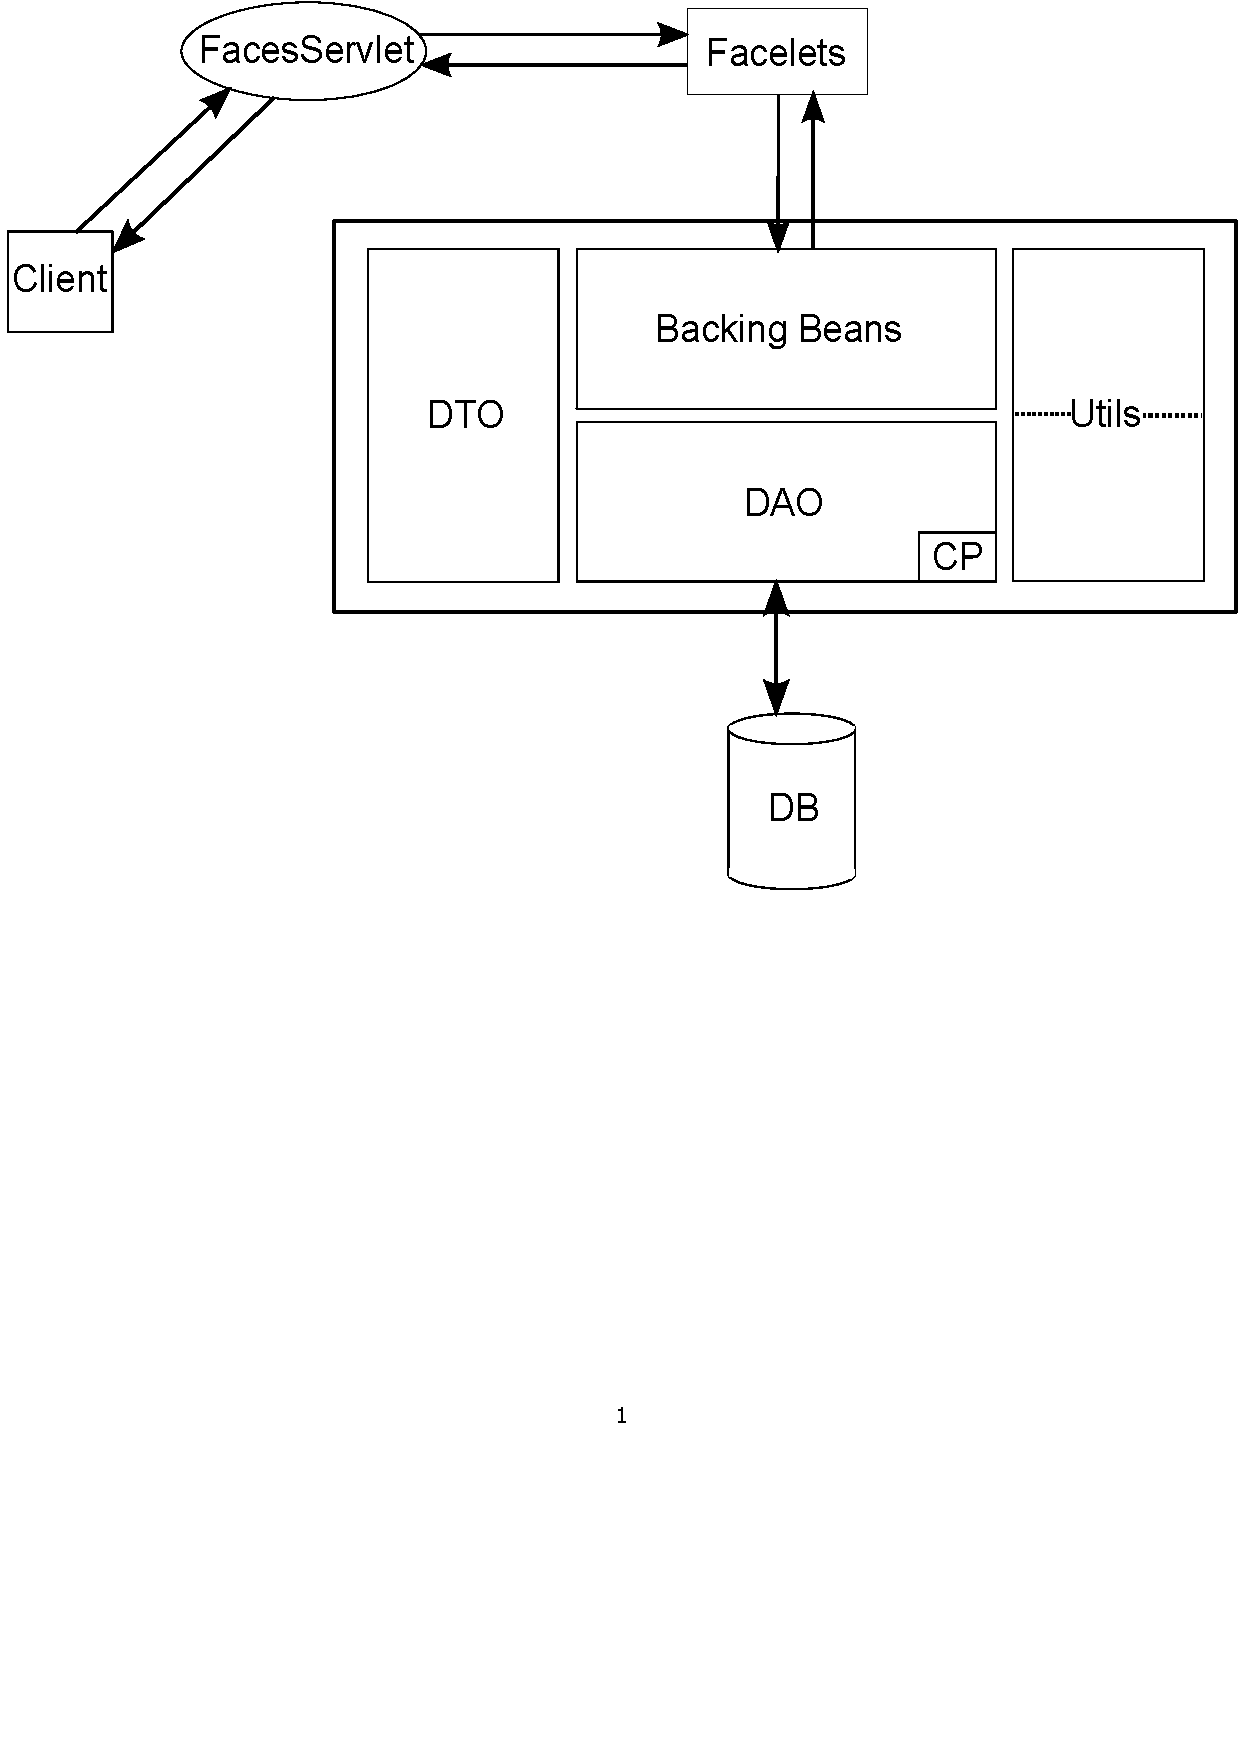
\includegraphics[scale=0.45]{Grafiken/Schichtenarchitektur.pdf}
	\subsection{Faces-Servlet}
	    Das Faces-Servlet fungiert im System als Controller, der eine HTTP-Request abfangt, diese bearbeitet, sowie weiterleitet. Das Faces-Servlet muss in jeder JSF-Applikation konfiguriert sein und wird in der web.xml Datei definiert. 
    \subsection{Facelets}
    	Die View wird durch Facelets repräsentiert. Es stellt den Inhalt dar, der vom Controller übergeben wird. Des Weiteren werden in der View die Benutzerinteraktionen entgegengenommen. 
   	\subsection{Model}
   	Das Model kann in vier Bereiche unterteilt werden. Die Upper Layer, welche die Backing Beans beinhalten, die Lower Layer mit den Data Access Objects (DAOs) und dem Connection Pool (CP), die Data Transfer Objects (DTOs) und den Utils. 
   		\subsubsection{Upper Layer}
   		Die "Upper Layer" besteht aus den Backing Beans. In Diesen ist zum Einen die Geschäftslogik enthalten, zum Anderen werden dort die überlieferten Benutzereingaben der Facelets übergeben, weiterverarbeitet und gespeichert.
    	\subsubsection{Lower Layer}
    	In der "Lower Layer" befinden sich die Data Access Objects und der Connection Pool. Mithilfe des CP greifen die DAOs auf die darunterliegende Database (DB) zu. 
    	\subsubsection{DTO}
    	Die Data Transfer Objects dienen als Schnittstelle zwischen den Backing Beans und den zugehörigen DAOs. Sie bündeln logisch zusammenhängende Daten in einem Objekt, um zeitintensive Fernzugriffe durch einen zu ersetzen.
    	\subsubsection{Utils}
    	Utils fungieren als Hilfs- und Verwalterklasse. Die Utils werden auch wiederum unterteilt, die man entweder den Backing Beans oder den DAOs zuordnen kann. 
    \subsection{Database}
    Die Database (DB) beinhaltet alle relevanten Daten, die für das System benötigt werden. Die DB kapselt die Daten von der Außenwelt ab, somit haben nur die DAOs haben Zugriff auf die DB. 
\section{Design Patterns}
Im Nachfolgendem werden die im System eingesetzten Design Patterns beschrieben.
	\begin{itemize}
		\item Data Transfer Object: Das DTO fassen mehrere Daten in einem Objekt zusammen, damit sie in einem Aufruf übergeben werden. Somit können Datensätze durch die Schichten transportiert werden.
		\item Dependency Injection: 
		\item Object Pooling:
		\item Creational Pattern:
			\begin{itemize}
				\item Factory Pattern:
				\item Singleton:
			\end{itemize}
		\item Singleton:
	\end{itemize}
\section{Fehlerbehandlung}		     

